\documentclass[t]{beamer}

\usepackage{biblatex}
\usepackage{algorithm}
\usepackage{src/templates/algorithmicx/algpseudocode}

\setbeamerfont{footnote}{size=\tiny}

\input{header-presentation}
\title[FPGA for BING!]{A Reconfigurable Fabric for Accelerating Large-Scale Datacenter Services}
\author[bobzhou@bu.edu]{Reviewed by Boyou Zhou}
\date[\today]{\today}

\begin{document}
\maketitle

\section*{FPGA for BING!}

\section{Intro: Why FPGA?}

\begin{frame}{What is ASIC, FPGA and GPP?}
    \begin{block}{ASIC}
        \begin{itemize}
            \item Application Specific Integrated Circuit
            \item Performance: Best, Cost: Highest, Time to Market: Slowest
        \end{itemize}
    \end{block}
    \begin{block}{FPGA}
        \begin{itemize}
            \item Field Programmable Gate Array
            \item Performance: Good, Cost: Normal, Time to Market: Normal 
        \end{itemize}
    \end{block}
    \begin{block}{GPP}
       \begin{itemize}
            \item General Purpose Processor
            \item Performance: Worst, Cost: Lowest, Time to Market: Fastest
       \end{itemize} 
    \end{block}
\end{frame}

\begin{frame}{Time to Market Comparison Between FPGA, and ASIC}
    \begin{figure}
        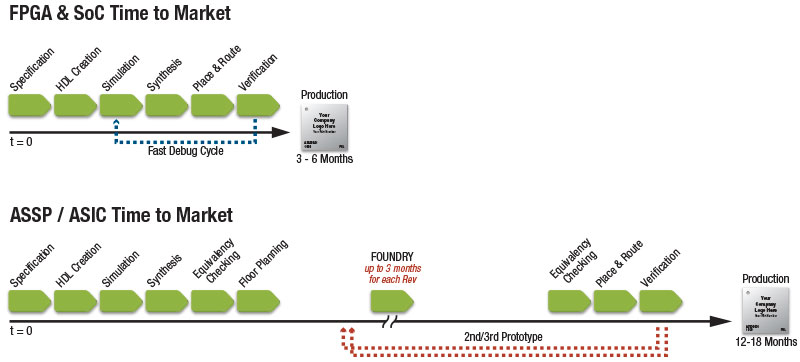
\includegraphics[width=4in]{img/design-time-comparison.png}
        \caption{Time to Market comparison\footcite{http://www.rtcmagazine.com/articles/view/102721}}
        \label{fig:time-to-market}
    \end{figure}
\end{frame}

\begin{frame}{Cost Comparison Between FPGA, and ASIC}
    \begin{figure}
        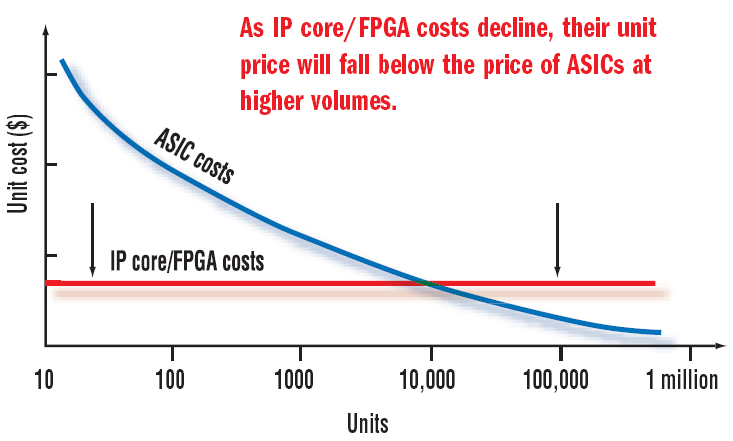
\includegraphics[width=2in]{img/FPGA-cost.png}~
        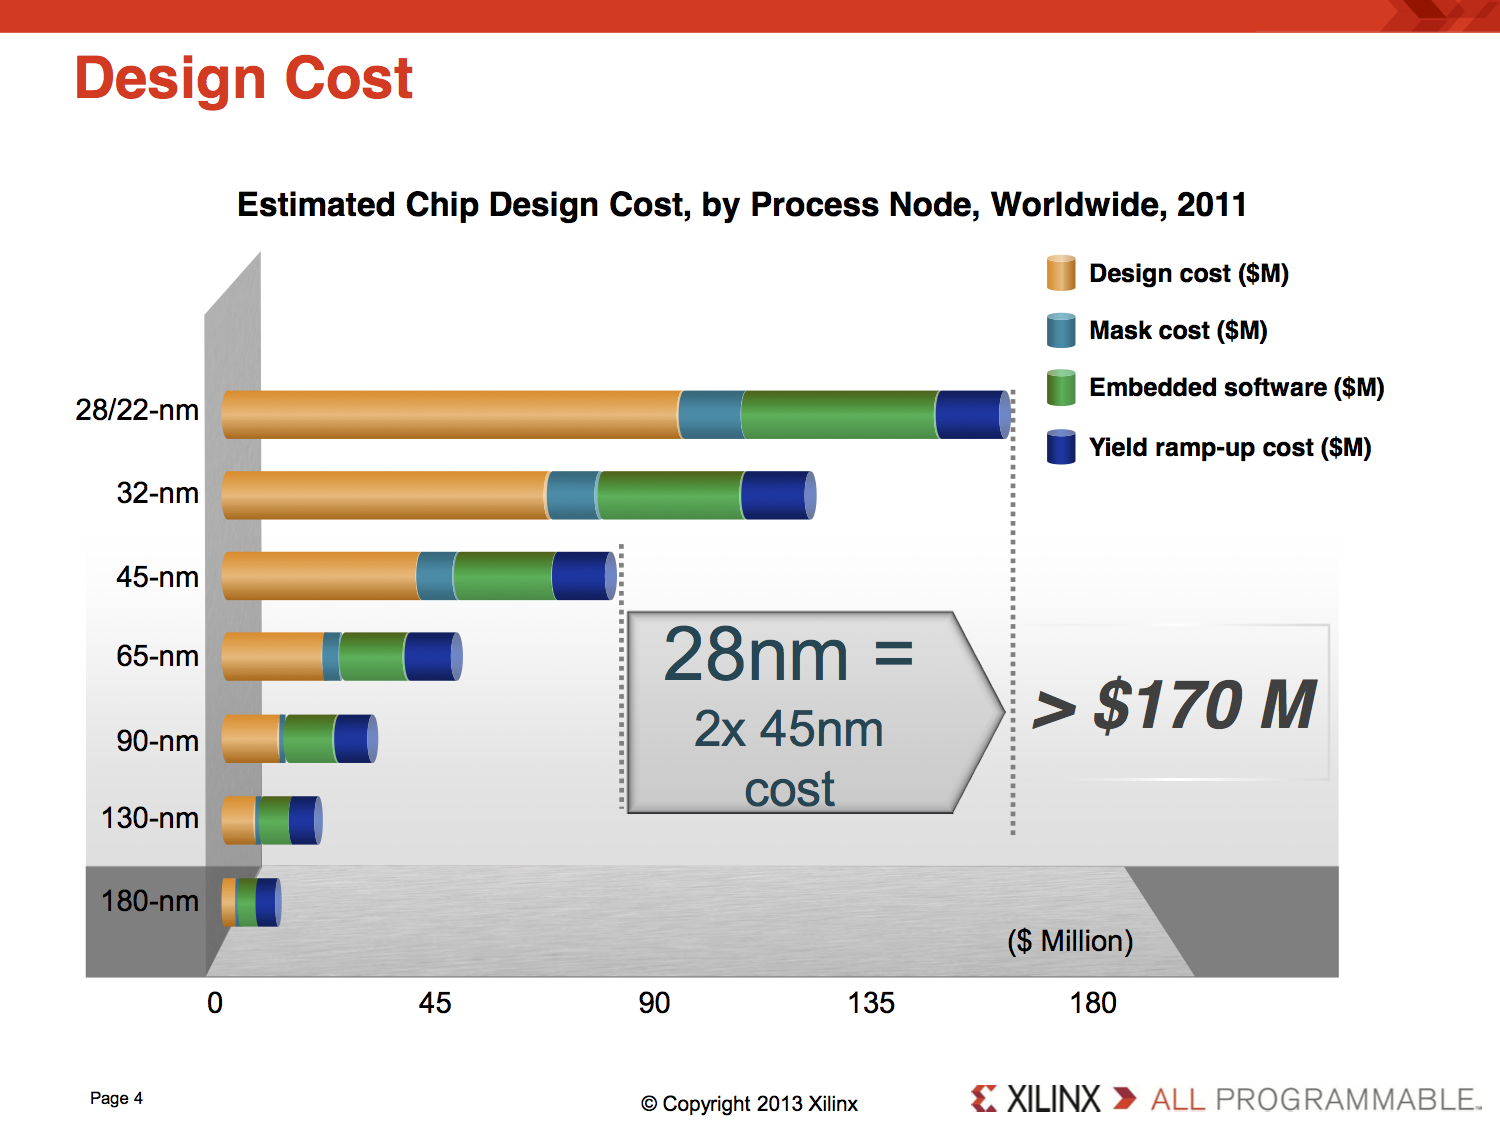
\includegraphics[width=2in]{img/ASIC-cost.png}
        \caption{FPGA cost\footcite{http://electronicdesign.com/files/29/12966/figure_01.gif}
                 ASIC cost\footcite{http://electroiq.com/blog/2014/02/semi-iss-scaling-innovation/}}
        \label{fig:cost-comparison}
    \end{figure}
\end{frame}

\begin{frame}{Performance Comparison Between GPP, FPGA, and ASIC}
    \begin{figure}
        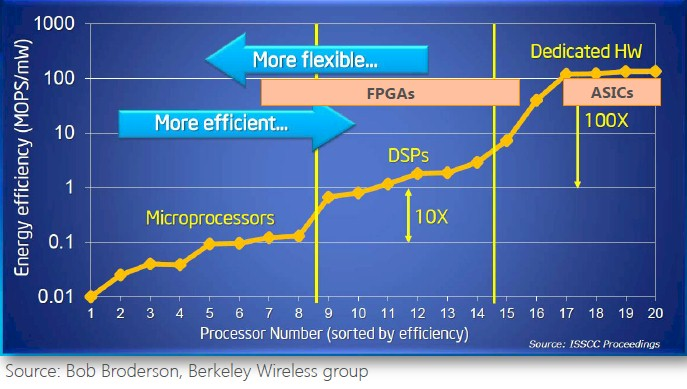
\includegraphics[width=4in]{img/microsoft-fpga-vs-cpu-vs-asic.png}
        \caption{FPGA, FPGA, and ASIC comparison from Microsoft\footcite{http://www.theplatform.net/2015/03/30/why-intel-might-buy-fpga-maker-altera}}
        \label{fig:performance-comparison}
    \end{figure}
\end{frame}

\section{Main Work: Use FPGA for Bing}
\begin{frame}{Main Work}
    \begin{block}{Resolved Problems}
        \begin{itemize}
            \item CPUs are too slow
        \end{itemize}
    \end{block}

    \begin{block}{Solution: reconfigurable Fabric, catapult Fabric}
        \begin{itemize}
            \item Each half-rack server is attached with a medium-sized FPGA and some DRAMs.
            \item FPGAs are wired to each other in 6x8 two-dimensional torus.
        \end{itemize}
    \end{block}

    \begin{block}{Evaluation: search requests from Bing}
        \begin{itemize}
            \item Softwares converts the documents to FPGA readable format, and then deliver the
            data to FPGA
            \item 2x throughput compared to software approach in the number of docs ranked per
            second per server
        \end{itemize}
    \end{block}
\end{frame}

\begin{frame}{Hardware Deployment}
    \begin{figure}
        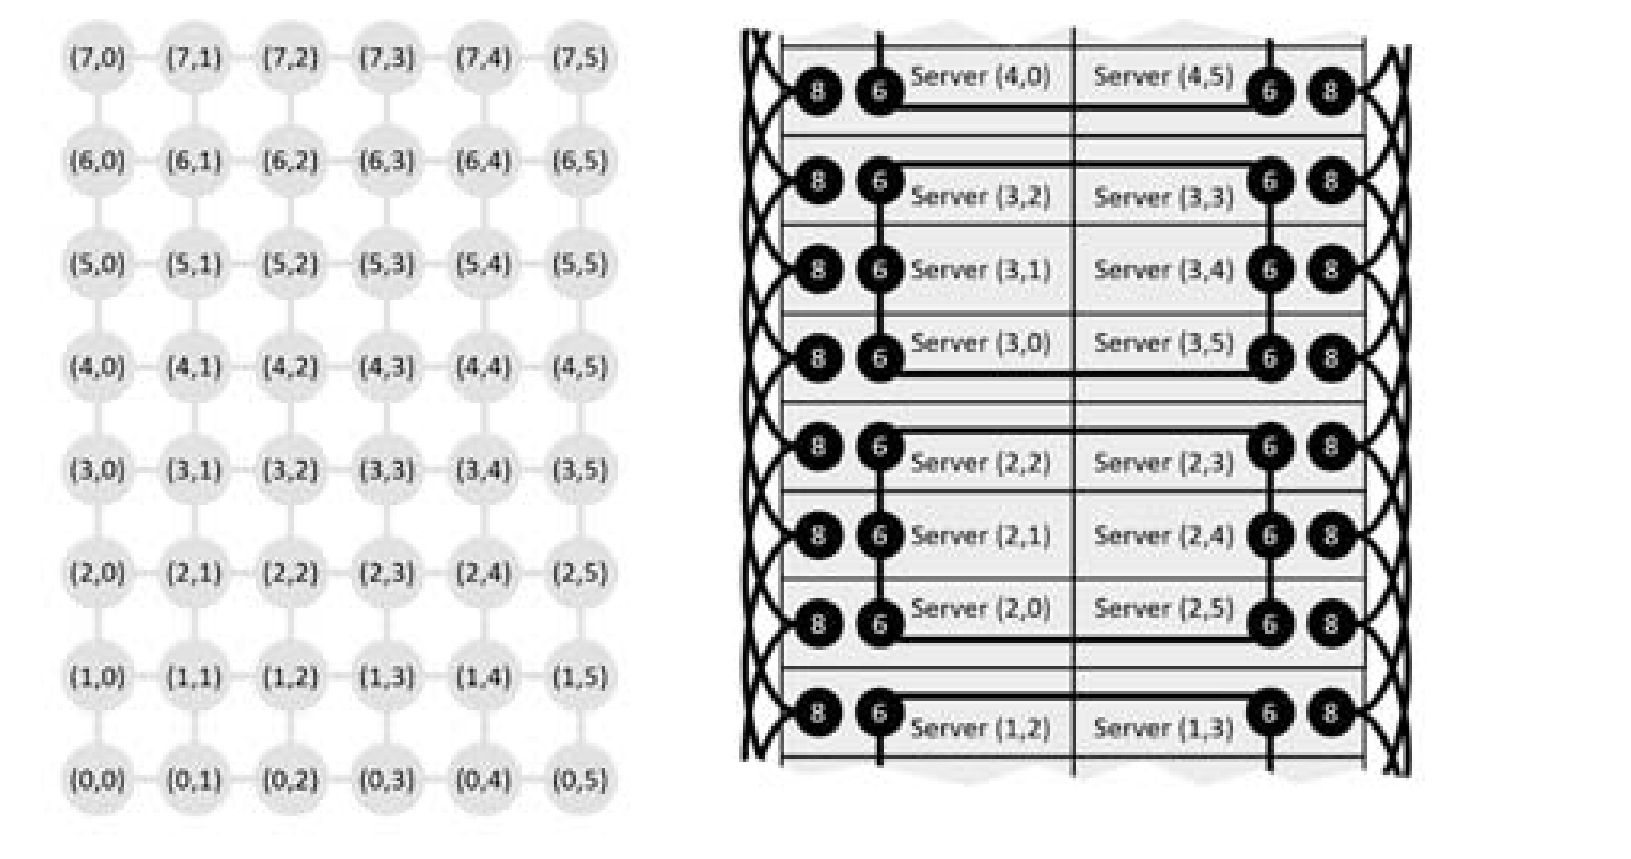
\includegraphics[width=4in]{img/torus-network.png}
        \caption{Logic mapping of the torus network}
        \label{fig:torus-network}
    \end{figure}
\end{frame}

\begin{frame}{Software Implementation}
    \begin{figure}
        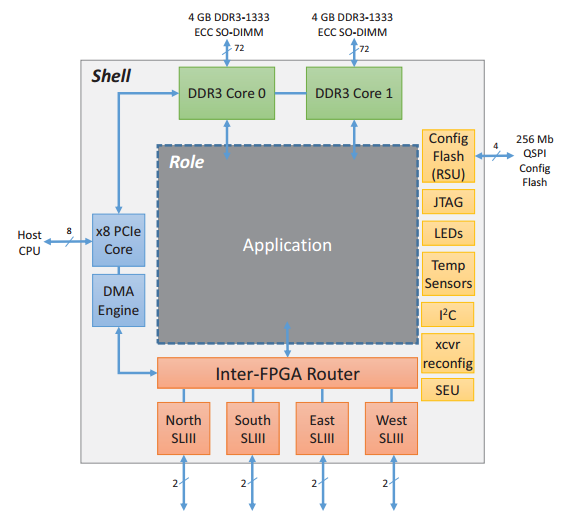
\includegraphics[width=2.5in]{img/shell-architecture.png}
        \caption{Shell Architecture}
        \label{fig:shell-architecture}
    \end{figure}
\end{frame}

\begin{frame}{Application Analysis}
    \begin{itemize}
        \item Data Arrives at Front-End cache service
        \item If a reuest is missed, it is routed to a top-level aggregator (TLA).
        \item TLA selects a machine.
        \item TLA sends the query to the machine.
        \item The machine performs a ranking service.
    \end{itemize}
\end{frame}

\section{How things are deployed}

\begin{frame}{Blocks Everywhere}
  \begin{block}{Blocks are better?}
    \begin{itemize}
    \item Everything in beamer seems to look better in blocks
    \item So, the default slide has a block and an itemized list
      \begin{itemize}
      \item You can also nest itemized lists
      \end{itemize}
    \end{itemize}
  \end{block}
\end{frame}

\begin{frame}{Column Slide}
  \begin{columns}[t]
    \column{0.60\textwidth}
    \begin{block}{First \textbf{BIG} Column}
      \begin{itemize}
      \item You can split content into columns
      \item Column size is governed manually
      \item Column alignment (here \texttt{b}, bottom) can also be specified
      \end{itemize}
    \end{block}

    \column{0.35\textwidth}
    \begin{block}{Second {\tiny little} Column}
      \begin{itemize}
      \item ALPHA
      \item BRAVO
      \item CHARLIE
      \item DELTA
      \item ECHO
      \end{itemize}
    \end{block}
  \end{columns}
\end{frame}
\end{document}
